\documentclass[aspectratio=169]{beamer} % 16:9 widescreen format
\usetheme{Madrid} % using the Madrid theme, you can choose another one if you prefer
\usecolortheme{beaver} % using the beaver color theme, you can choose another one if you prefer
\usepackage{graphicx}
\usepackage{hyperref} % to use \url
\usepackage{tikz}
\usepackage{adjustbox}

\usetikzlibrary{shapes.geometric, arrows}
\tikzstyle{startstop} = [rectangle, rounded corners, 
minimum width=3cm, 
minimum height=1cm,
text centered, 
draw=black, 
fill=red!30]

\tikzstyle{io} = [trapezium, 
trapezium stretches=true, 
trapezium left angle=70, 
trapezium right angle=110, 
minimum width=3cm, 
minimum height=1cm, text centered, 
draw=black, fill=blue!30]

\tikzstyle{process} = [rectangle, 
minimum width=3cm, 
minimum height=1cm, 
text centered, 
text width=3cm, 
draw=black, 
fill=orange!30]

\tikzstyle{decision} = [diamond, 
minimum width=3cm, 
minimum height=1cm, 
text centered, 
draw=black, 
fill=green!30]
\tikzstyle{arrow} = [thick,->,>=stealth]
\usepackage{xeCJK} 
\setbeamertemplate{footline}[page number] % removes the footer except for the slide count
\setbeamertemplate{navigation symbols}{} % removes navigation symbols

\title{Exploring Parallelism Opportunities in KLayout}
\subtitle{A Journey of Learning with Open Source EDA Software}
\author{Group 22: 陳則仁 \& 鄢銘宏}
\date{\today}

\begin{document}

\begin{frame}
    \titlepage
\end{frame}
    
\begin{frame}{KLayout}
    \begin{columns}[T]
        \begin{column}{.6\textwidth}
        \begin{itemize}
            \item \textbf{About KLayout:}
                \begin{itemize}
                    \item A open source (GPL 3.0) project started as a viewer, then editor/analyzer/multitool 
                    \item First released in 2006-04; By Matthias \textbf{K}oefferlein
                    \item Cross platform (Linux distros/Windows/MacOSX) achieved by QT, compact  <100MB installation
                    \item Users from Google open source PDK project, special manufacturing process like photonic, quantum computer. Also widely used by personnels in the EDA (Electrical Design Automation) industry.
                    \item Commercial alternatives include Virtuoso(CDNS) or Laker(Was Spring-Soft, later acquired by SNPS) for layout/schematic editing/viewing, Calibre(Siemens EDA) for physical verification
                \end{itemize}
        \end{itemize}
        \end{column}
        \begin{column}{.4\textwidth}
        \includegraphics[width=\textwidth,height=\textheight,keepaspectratio]{klayout.png}
        \end{column}
    \end{columns}
\end{frame}

\begin{frame}{Project Goals}
    \begin{columns}[T]
        \begin{column}{.6\textwidth}
            \begin{itemize}
                \item Apply parallel programming techniques to improve runtime of KLayout's Design Rule Check (DRC) operation
                \item Gain insights from a substantial, real-world C++ code base \linebreak (\texttt{git ls-files |grep ".cc"| xargs wc -l} yields 2,688,261 lines of code)
                \item Explore and learn from the open-source EDA ecosystem
            \end{itemize}
        \end{column}
        \begin{column}{.4\textwidth}
            \begin{adjustbox}{max totalsize={.95\textwidth},center}
                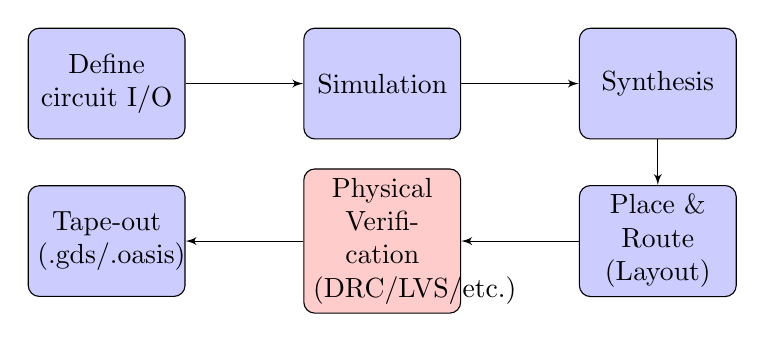
\begin{tikzpicture}[node distance=2cm, auto]
                    % Define styles for boxes and line
                    \tikzstyle{block} = [rectangle, draw, fill=blue!20, text width=5em, text centered, rounded corners, minimum height=4em]
                    \tikzstyle{emph_block} = [block, fill=red!20]  % emphasize block
                    \tikzstyle{line} = [draw, -latex']
            
                    % Place nodes
                    \node [block] (sys_spec) {Define circuit I/O};
                    \node [block, right of=sys_spec, node distance=3.5cm] (simulation) {Simulation};
                    \node [block, right of=simulation, node distance=3.5cm] (synthesis) {Synthesis};
                    \node [block, below of=synthesis, node distance=2cm] (place_route) {Place \& Route\linebreak (Layout)};
                    \node [emph_block, left of=place_route, node distance=3.5cm] (phy_verify) {Physical Verification \linebreak (DRC/LVS/etc.)};
                    \node [block, left of=phy_verify, node distance=3.5cm] (tape_out) {Tape-out \linebreak (.gds/.oasis)};
            
                    % Draw edges
                    \path [line] (sys_spec) -- (simulation);
                    \path [line] (simulation) -- (synthesis);
                    \path [line] (synthesis) -- (place_route);
                    \path [line] (place_route) -- (phy_verify);
                    \path [line] (phy_verify) -- (tape_out);
                \end{tikzpicture}
            \end{adjustbox}
        \end{column}
    \end{columns}
\end{frame}



\begin{frame}{Inputs: Layers, Polygons, and Cells}
    \begin{columns}[T]
        \begin{column}{.6\textwidth}
        \begin{itemize}
        \item \textbf{Layer:} Layers in a GDSII or OASIS layout input can be visualized as a stack of transparent films, each containing different geometries.
        \item \textbf{Polygon:} The fundamental building blocks of the layout are polygons, basic shapes that are used to form more complex structures, it consists of points at 2D plane.
        \item \textbf{Cell:} A cell can contain multiple layers with different polygons, forming a hierarchical structure in the layout design.
        \end{itemize}
        \end{column}
        \begin{column}{.4\textwidth}
            \includegraphics[width=\textwidth,height=0.8\textheight,keepaspectratio]{cmos_logics.png}
        \end{column}
    \end{columns}
\end{frame}



\begin{frame}{Example DRC Rules (Skywater 130)}
    \begin{columns}[T]
        \begin{column}{1.0\textwidth}
            \begin{itemize}
                \item \texttt{poly.not(diff).edges.and(gate.and(lvtn).edges).space(0.35, euclidian).output("poly.1b", "poly.1b: min. lvtn gate width : 0.35um")}
                \item \texttt{poly.isolated(0.21, euclidian).output("poly.2", "poly.2 : min. poly spacing : 0.21um")}
                \item \texttt{poly.and(rpm.or(urpm).or(poly\_rs)).width(0.33, euclidian).output("poly.3", "poly.3 : min. poly resistor width : 0.33um")}
            \end{itemize}
            These rules can serve as examples to understand the layout of DRC rules. DRC rules are written in a domain-specific language, which allows expressing complex geometric constraints in a compact and readable way. In these examples, geometric operations are combined with logical operations to describe the required conditions on layout layers.
        \end{column}
    \end{columns}
\end{frame}


\begin{frame}{Results of "and" operation}
    \begin{center}
        \includegraphics[width=\textwidth,height=0.8\textheight,keepaspectratio]{and.png}
    \end{center}
\end{frame}

\begin{frame}{Test case from SkyWater 130 Process and Open Source IC Design}
    \begin{columns}[T]
        \begin{column}{.6\textwidth}
        \begin{itemize}
        \item \textbf{SkyWater 130 Process:} An open-source semiconductor process for designing custom ICs. SkyWater 130nm provides a PDK for creating manufacturable designs.
        \item \textbf{Google Open Source IC design project:} Google and efabless have partnered to produce open source designs that can be manufactured using the SkyWater 130 process.
        \item \textbf{Test Case:} Many Caravel RISC-V test cases can be found at github.
        \end{itemize}
        \end{column}
        \begin{column}{.4\textwidth}
        \includegraphics[width=\textwidth,height=0.8\textheight,keepaspectratio]{caravel.png}
        \end{column}
    \end{columns}
    \end{frame}
    \begin{frame}{Proposed Solutions}
        \begin{columns}[T]
            \begin{column}{.6\textwidth}
            \begin{itemize}
                \item \textbf{OpenMP:} 
                \begin{itemize}
                    \item \textit{Benefits:} 
                        \begin{itemize}
                            \item Easy to integrate into existing code.
                        \end{itemize}
                    \item \textit{Drawbacks:}
                        \begin{itemize}
                            \item Requires careful management of shared data to avoid race conditions.
                            \item Not successful in this particular scenario.
                        \end{itemize}
                \end{itemize}
                
                \item \textbf{TaskFlow:} Task, DRC operation level parallelism.
                \begin{itemize}
                    \item \textit{Benefits:}
                        \begin{itemize}
                            \item Provides more fine-grained control over parallelism compared to OpenMP.
                            \item Can express complex dependencies between tasks.
                        \end{itemize}
                    \item \textit{Drawbacks:}
                        \begin{itemize}
                            \item More complex to set up and manage compared to OpenMP.
                            \item Work-in-progress for this particular scenario.
                        \end{itemize}
                \end{itemize}
            \end{itemize}
            \end{column}
            \begin{column}{.4\textwidth}
            \begin{center}
                \includegraphics[width=\textwidth,height=0.8\textheight,keepaspectratio]{solutions.png}
            \end{center}
            \end{column}
        \end{columns}
    \end{frame}
    

\begin{frame}{Lessons Learned from OpenMP and Klayout DRC}
    \begin{columns}[T]
        \begin{column}{.6\textwidth}
            \begin{itemize}
                \item Objectives: Attempted to improve the runtime of ``gate = poly.and(diff)'' operation of caravel test case. '(~5 Million gate shapes)'
                \item Challenges faced:
                    \begin{itemize}
                        \item Code is hard to trace. RBI calls Cpp code with templates, overrides, delegate patterns. One segment of code is shared by many DRC commands (and, or implementations are shared).
                        \item Used gdb/perf+flameGraph to understand where the slowest part is.
                        \item Iterator pattern is widely used, making it difficult to apply parallel for pragma. Once found a for loop in the scanline algorithm in and\_or operation that seemed to be a good parallel for candidate but later turned out that part of code is not reentrant/thread safe.
                    \end{itemize}
            \end{itemize}

        \end{column}
        \begin{column}{.4\textwidth}
            \begin{center}
                \includegraphics[width=\textwidth,height=0.8\textheight,keepaspectratio]{flame.png}
            \end{center}
        \end{column}
    \end{columns}
\end{frame}




\begin{frame}{Work in Progress with TaskFlow + Klayout DRC}
    \begin{columns}[T]
        \begin{column}{.6\textwidth}
        \begin{itemize}
            \item TaskFlow allows for easy task management by simply declaring them, while effectively handling parallelism.
            \item Given that DRC rules are largely independent and can be modeled as distinct tasks, TaskFlow offers a promising approach to enhance runtime without requiring extensive modification to the Klayout code base.
        \end{itemize}
        \end{column}
        \begin{column}{.4\textwidth}
        \begin{center}
            \includegraphics[width=\textwidth,height=0.8\textheight,keepaspectratio]{taskflow.png}
        \end{center}
        \end{column}
    \end{columns}
\end{frame}





\begin{frame}{KLayout Code with TaskFlow}
    \begin{itemize}
        \item This is an example of KLayout's C++ code that utilizes TaskFlow.
        \item Compared to the sequential version, there is approximately a 4X improvement in runtime.
    \end{itemize}
    \begin{center}
        \includegraphics[width=\textwidth,height=0.8\textheight,keepaspectratio]{klayout_taskflow.png}
    \end{center}
\end{frame}

\begin{frame}{Conclusion and Future Work}
    \begin{itemize}
        \item The KLayout DRC operation can leverage parallel programming techniques for enhanced performance.
        \item While OpenMP provided a good starting point, it proved challenging due to the complexities inherent to the codebase.
        \item TaskFlow demonstrates potential in achieving task/DRC operation level parallelism.
        \item Future work encompasses continued implementation of TaskFlow, parsing Ruby code into syntax trees to generate C++ TaskFlow-based KLayout DRC code, and further exploration of the codebase to uncover additional parallelism opportunities.
    \end{itemize}
\end{frame}


\begin{frame}{Q \& A}
    \begin{center}
        Thank you for your attention! Questions?
    \end{center}
\end{frame}



\end{document}
